\documentclass{ctexbeamer}

\usepackage{graphicx}
\usepackage{hyperref}

\usetheme{Berkeley}
\beamertemplatenavigationsymbolsempty

\title{下一代如意包管理器进展介绍}
\author{NickCao}
\date{2023年6月27日}

\begin{document}
\frame{\titlepage}

\section{why}

\begin{frame}
  \frametitle{假如我们需要搭建一套RISC-V开发环境}
  \begin{figure}
    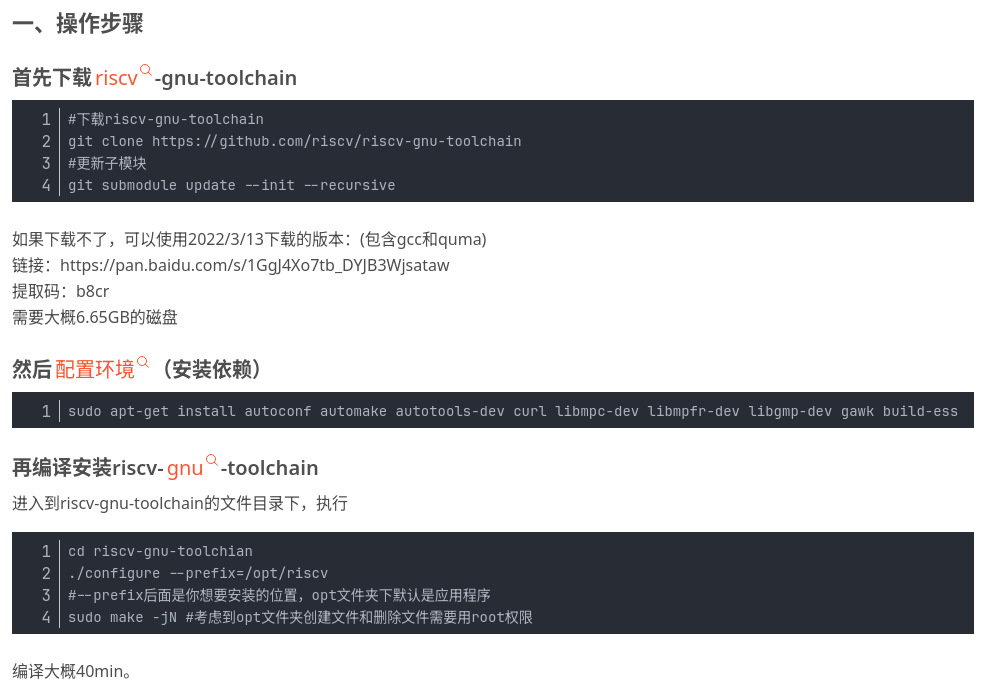
\includegraphics[width=\linewidth]{./csdn-1.png}
  \end{figure}
\end{frame}

\begin{frame}
  \frametitle{假如我们需要搭建一套RISC-V开发环境}
  \begin{figure}
    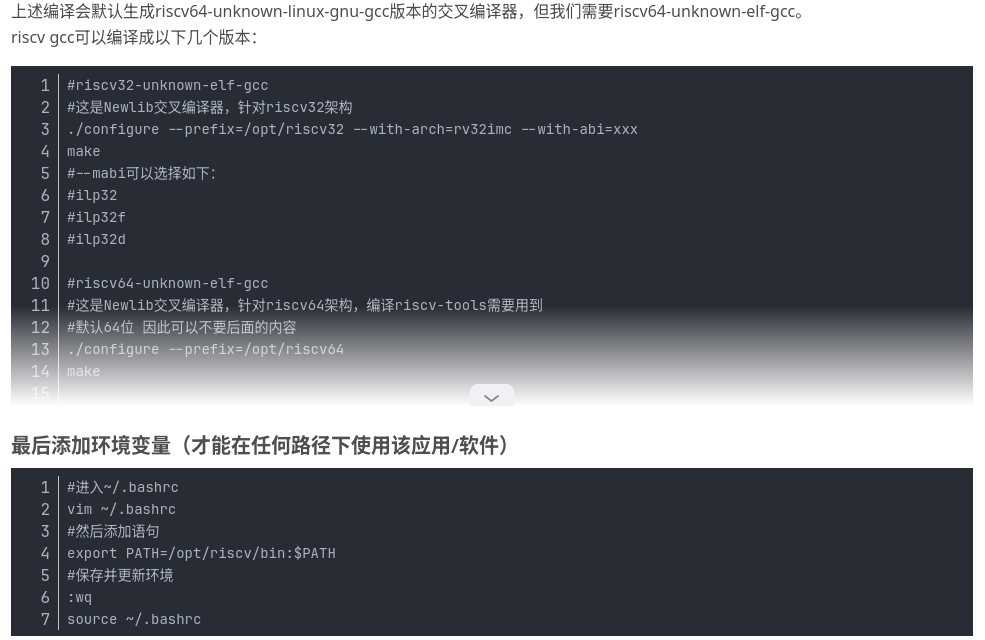
\includegraphics[width=\linewidth]{./csdn-2.png}
  \end{figure}
\end{frame}

\begin{frame}
  \frametitle{为什么要用包管理}
  \begin{exampleblock}{另一种可能}
    \texttt{ruyi package add riscv-gnu-toolchain}
  \end{exampleblock}
  \begin{columns}
    \begin{column}{0.65\linewidth}
      \begin{description}
        \item[方便快捷] 无需处理依赖\footnotemark[1]或编译
        \item[生命周期] 随时获得最新版本
        \item[质量控制] 没有配置出错的后顾之忧
      \end{description}
      \footnotetext[1]{图为pacvis绘制的软件包依赖关系图}
    \end{column}
    \begin{column}{0.35\linewidth}
      \begin{figure}
        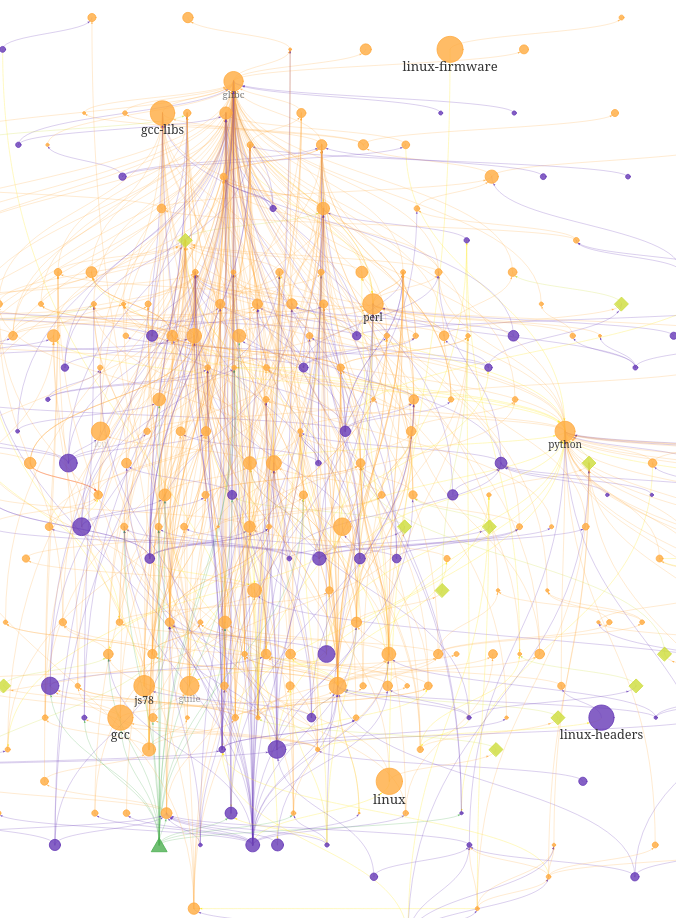
\includegraphics[width=\linewidth]{./pacviz.png}
      \end{figure}
    \end{column}
  \end{columns}
\end{frame}

\begin{frame}
  \frametitle{为什么又要做一个包管理}
  \begin{block}{Conda}
    \begin{itemize}
      \item 依赖解析速度慢
      \item 打包质量堪忧
    \end{itemize}
  \end{block}
  \begin{figure}
    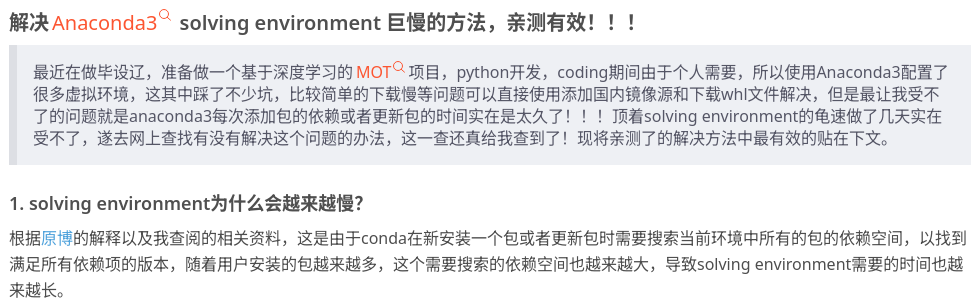
\includegraphics[width=\linewidth]{./csdn-conda.png}
  \end{figure}
\end{frame}

\begin{frame}
  \frametitle{为什么又要做一个包管理}
  \begin{block}{apt/dnf/pacman}
    \begin{itemize}
      \item 仅能在单一发行版上工作
      \item 各大发行版的包各不相同
    \end{itemize}
  \end{block}
  \begin{figure}
    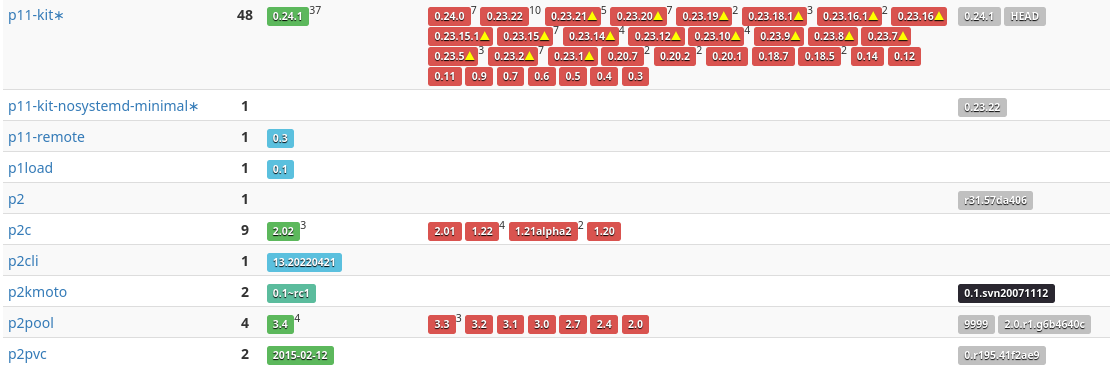
\includegraphics[width=\linewidth]{./repology.png}
  \end{figure}
\end{frame}

\begin{frame}
  \frametitle{为什么又要做一个包管理}
  \begin{block}{Docker\footnote{并不是包管理}}
    \begin{itemize}
      \item 无法使用主机上已经安装的工具
      \item 访问GPU等硬件往往需要复杂的配置
    \end{itemize}
  \end{block}
  \begin{block}{Spack/Gentoo Prefix}
    \begin{itemize}
      \item 多不提供二进制包,仍需要编译
      \item 使用较为繁琐,学习曲线陡峭
    \end{itemize}
  \end{block}
\end{frame}

\section{what}

\begin{frame}
  \frametitle{我们想要怎样的包管理}
  \begin{description}
    \item[简单易于使用] 无需学习即可快速上手
    \item[跨发行版工作] 无论是Ubuntu、CentOS还是WSL都能使用
    \item[建立隔离环境] 不同项目开发环境互不干扰
    \item[可用软件包多] 开发各类项目都能得心应手
    \item[\textbf{多年后还工作}] 无论过了多久,同样的开发环境仍可重现
  \end{description}
  \begin{figure}
    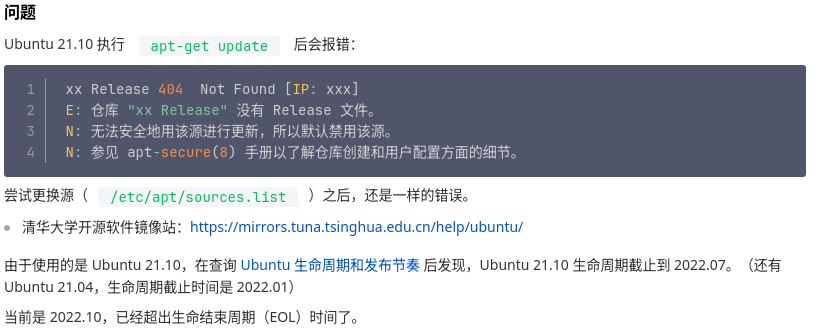
\includegraphics[width=\linewidth]{./csdn-404.png}
  \end{figure}
\end{frame}

\begin{frame}{我们有这样的包管理吗}
  \begin{exampleblock}{有}
    Nix
  \end{exampleblock}
  \begin{itemize}
    \item 跨发行版,乃至macOS和OpenBSD工作
    \item 可以建立隔离环境,同个软件包的不同版本也可共存
    \item 源码与二进制混合发行,便于自定义
    \item 目前为世界上软件包数量遥遥领先的发行版
    \item 十五年前的软件包依然工作\footnote{\url{https://blinry.org/nix-time-travel/}}
  \end{itemize}
  \begin{alertblock}{但是}
    学习曲线过于陡峭,non-FHS的设计与闭源软件等并不兼容
  \end{alertblock}
\end{frame}

\section{how}
\begin{frame}
  \frametitle{我们如何构建一个这样的包管理}
  \begin{figure}
    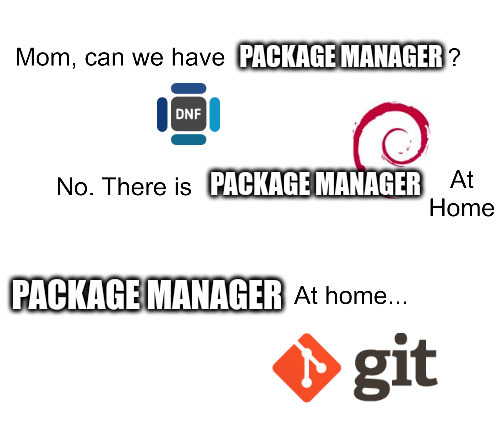
\includegraphics[width=0.8\linewidth]{./meme.jpg}
  \end{figure}
\end{frame}

\begin{frame}
  \frametitle{我们如何构建一个这样的包管理}
  \begin{exampleblock}{Git}
    \begin{itemize}
      \item 包管理的本质就是把指定文件放到指定位置
      \item 使用环境:git checkout base
      \item 创建环境:git checkout -b develop
      \item 安装软件:git cherry-pick gcc
      \item 保存环境:git commit -m "installed gcc"
      \item 分享环境:git pull/push
    \end{itemize}
  \end{exampleblock}
  \begin{alertblock}{但是}
    Git并不适合管理二进制文件
  \end{alertblock}
\end{frame}

\begin{frame}
  \frametitle{我们如何构建一个这样的包管理}
  \begin{exampleblock}{OSTree\footnotemark[2]}
    \begin{itemize}
      \item 专为二进制文件设计的Git
      \item content addresses存储,自动去重
      \item 可以使用容器镜像服务存储数据
    \end{itemize}
  \end{exampleblock}
  \begin{alertblock}{但是}
    里面的东西哪里来
  \end{alertblock}
  \begin{block}{元包管理}
    不如我们把现有的东西塞进去
  \end{block}
  \footnotetext[2]{\url{https://ostreedev.github.io/ostree/}}
\end{frame}

\begin{frame}
  \frametitle{现有的东西}
  \begin{figure}
    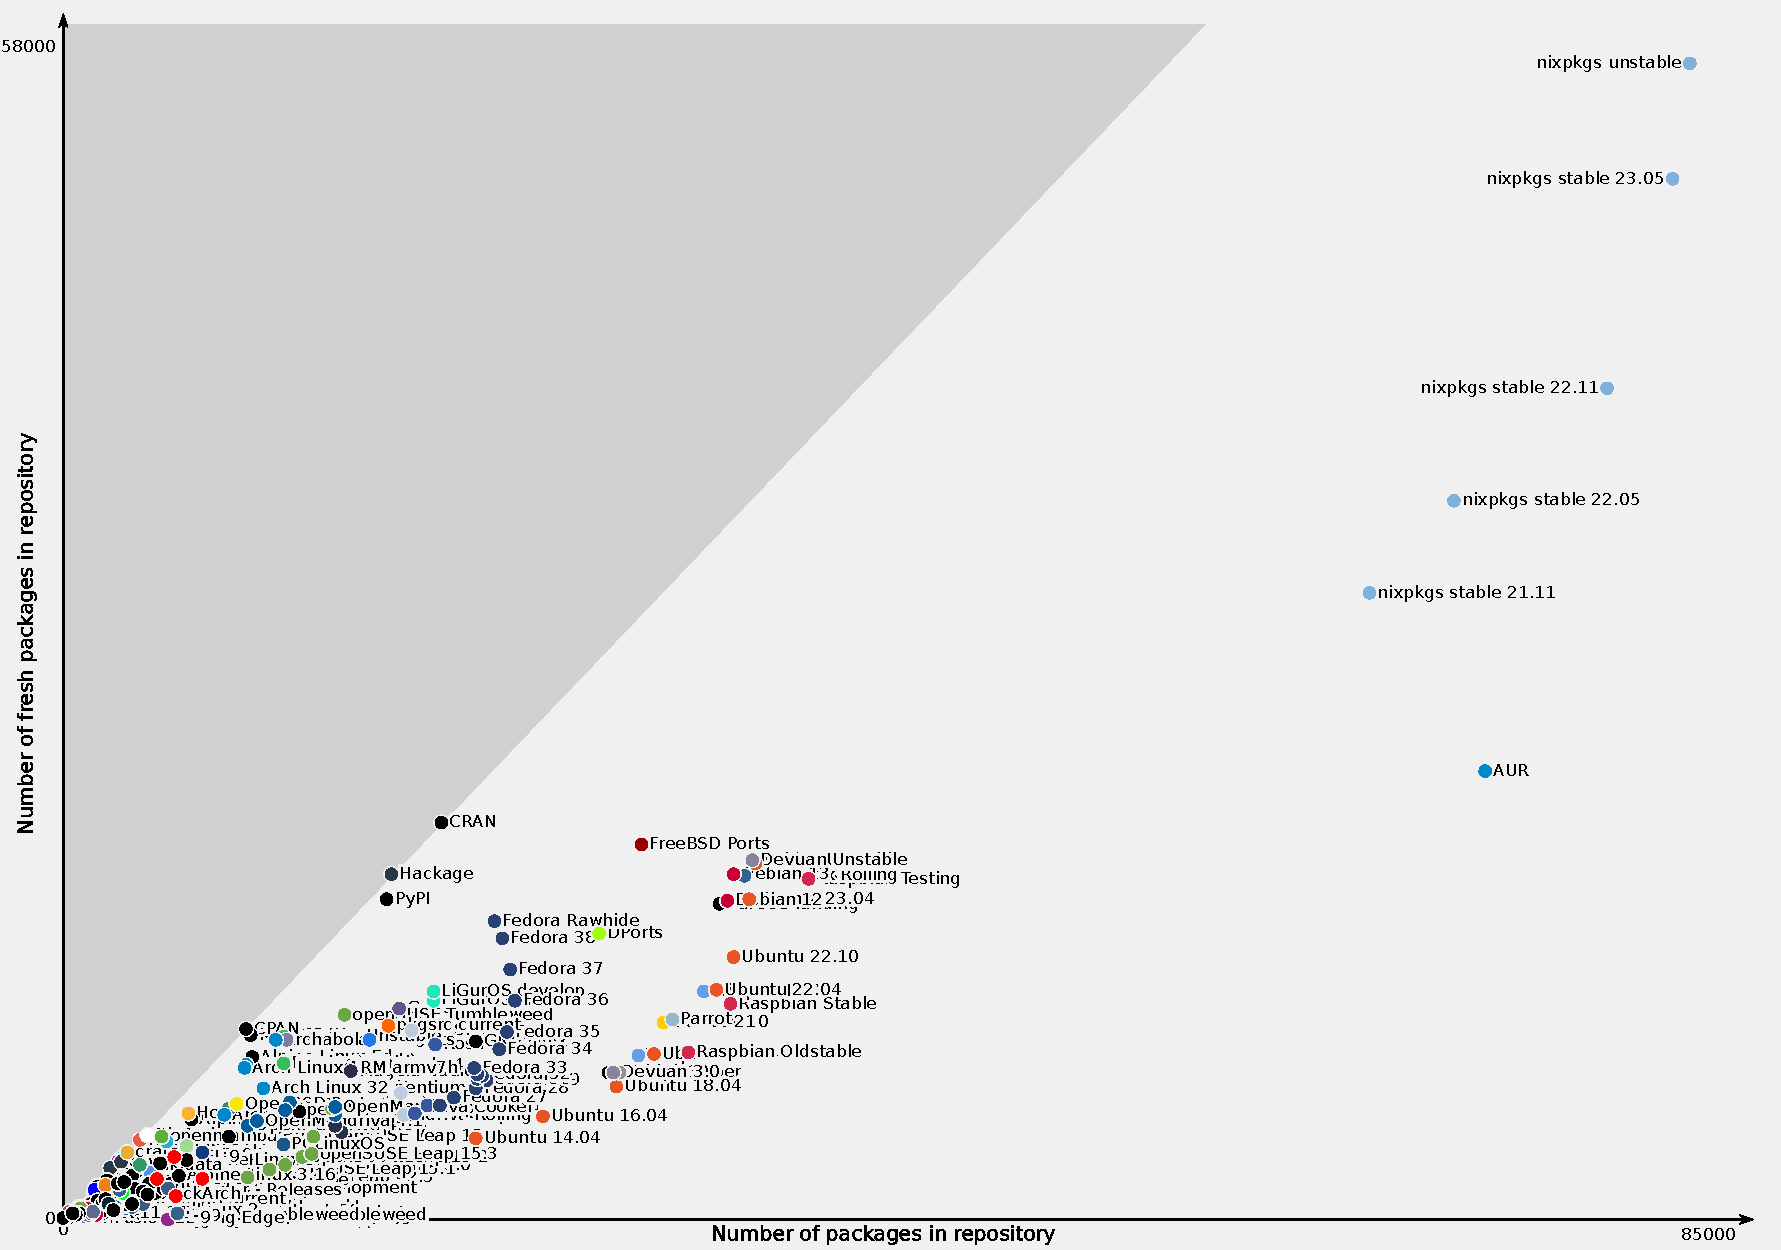
\includegraphics[width=\linewidth]{./map_repo_size_fresh.pdf}
  \end{figure}
\end{frame}

\begin{frame}[fragile]
  \frametitle{我们试图构建一个这样的包管理}
  \begin{block}{第一次尝试}
    直接把一个现有的发行版解压到一个目录里
  \end{block}
  \begin{small}
  \begin{verbatim}
  $ tar xf archlinux.tar.gz -C /opt/arch/
  $ /opt/arch/bin/ls
  bash: ls: cannot execute: required file not found
  # 动态链接的二进制程序需要解释器才能执行
  $ patchelf --print-interpreter /opt/arch/bin/ls
  /lib64/ld-linux-x86-64.so.2
  \end{verbatim}
  \end{small}
\end{frame}

\begin{frame}[fragile]
  \frametitle{我们好像构建出了一个这样的包管理}
  \begin{block}{第二次尝试}
    解压后再做点修改
  \end{block}
  \begin{small}
  \begin{verbatim}
  $ patchelf --set-interpreter \
      /opt/arch/lib64/ld-linux-x86-64.so.2 \
      /opt/arch/bin/ls
  $ /opt/arch/bin/ls
  /opt/arch/bin/ls: error while loading shared
  libraries: libcap.so.2: cannot open shared object
  file: No such file or directory
  $ patchelf --set-rpath /opt/arch/lib /opt/arch/bin/ls
  $ /opt/arch/bin/ls
  Documents  Downloads  Pictures  Projects
  \end{verbatim}
  \end{small}
\end{frame}

\begin{frame}
  \frametitle{我们好像构建出了一个这样的包管理}
  \begin{alertblock}{但是}
    软件包中不只有ELF,还有头文件、资源文件、配置文件\dots
  \end{alertblock}
  \begin{exampleblock}{chroot}
    让文件在它原本该在的地方
  \end{exampleblock}
  \begin{itemize}
    \item 首先把一个发行版的镜像解压到某个地方
    \item 然后chroot进去
    \item 我们成功发明了:Docker
  \end{itemize}
  \begin{block}{为什么我们不喜欢Docker}
    我们想要隔离的环境,但我们不想要隔离
  \end{block}
\end{frame}

\begin{frame}
  \frametitle{我们如何构建一个这样的包管理}
  我们需要一个支持在prefix下运行的发行版
  \begin{exampleblock}{Gentoo Prefix}
    To bring out the virtues of Gentoo Linux on different operating systems, the Gentoo Prefix project develops and maintains a way of installing Gentoo systems in a non-standard location, designated by a "prefix".
  \end{exampleblock}
  \begin{block}{Fedora (or generally, rpm)}
    \url{https://docs.fedoraproject.org/en-US/packaging-guidelines/\#\_relocatable_packages}
  \end{block}
\end{frame}

\begin{frame}[fragile]
  \frametitle{我们如何构建一个这样的包管理}
  我们也可以先将就一下
  \begin{exampleblock}{bubblewrap}
    Low-level unprivileged sandboxing tool used by Flatpak and similar projects
  \end{exampleblock}
  \begin{small}
  \begin{verbatim}
  $ bwrap \
     --bind /opt/arch / \
     --bind /home /home \
     /usr/bin/ls
  Documents  Downloads  Pictures  Projects
  \end{verbatim}
  \end{small}
\end{frame}

\begin{frame}
  \frametitle{我们如何构建一个这样的包管理}
  \begin{itemize}
    \item 简单易于使用
    \item 跨发行版工作 \checkmark
    \item 建立隔离环境 \checkmark
    \item 可用软件包多 \checkmark
    \item 多年后还工作
  \end{itemize}
\end{frame}

\begin{frame}
  \frametitle{我们如何构建一个这样的包管理}
  \begin{block}{简单易于使用}
    \begin{itemize}
      \item 为各发行版建立一套统一的基线环境
      \item 为各种语言和框架提供预构建的开发套件
    \end{itemize}
  \end{block}
  \begin{block}{多年后还工作}
    \begin{itemize}
      \item 为各发行版提供历史镜像
      \item 使用类似Dockerfile的形式创建开发环境
    \end{itemize}
  \end{block}
\end{frame}

\begin{frame}[fragile]
  \frametitle{我们如何构建一个这样的包管理}
  \begin{itemize}
    \item 保存每个发行版的软件仓库每天的状态
    \item 基于发行版仓库元数据锁定文件哈希
    \item 对外提供和普通镜像源一致的http访问
    \item 无需修改包管理器,仅修改镜像地址即可回到任意一天
  \end{itemize}
  \begin{verbatim}
    FROM ubuntu:2023-06-27
    LANGUAGE rust haskell c++
    FRAMEWORK boost qt6
    PACKAGE msgpack-cxx doxygen
  \end{verbatim}
\end{frame}

\begin{frame}[fragile]
  \frametitle{下一代如意包管理器}
  \begin{verbatim}
  # 初始化如意
  $ ruyi init
  # 拉取基础镜像
  $ ruyi pull example.com/archlinux
  # 建立工作副本
  $ ruyi checkout example.com/archlinux develop
  # 激活开发环境
  $ ruyi activate develop
  # 对环境进行修改
  $ ruyi framework add qt6
  $ pacman -S nano
  # 提交改动
  $ ruyi commit develop example.com/archlinux-new
  $ ruyi push example.com/archlinux-new
  \end{verbatim}
\end{frame}

\begin{frame}
  \frametitle{下一代如意包管理器}
  
\includegraphics[width=\linewidth]{./ruyi-meme.jpg}
\end{frame}

\begin{frame}
  \frametitle{下一代如意包管理器}
  \begin{itemize}
    \item 基于OSTree与bubblewrap打造
    \item 提供一个类似Docker与Conda的易用的cli界面
    \item 手动创建环境与Ruyifile声明式构建两种工作模式
    \item 长期可用的历史镜像确保可复现性
  \end{itemize}
  \begin{exampleblock}{Bonus}
    为如意而建立的镜像存储服务与cli也可用于管理非如意创建的系统镜像,为目前的工作流提供帮助
  \end{exampleblock}
  \begin{figure}
    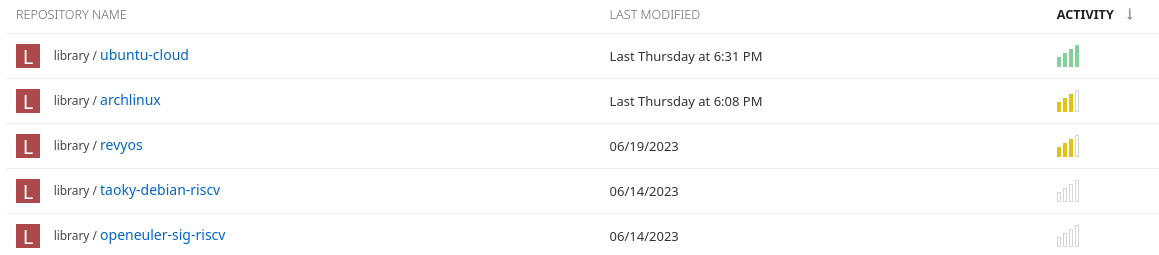
\includegraphics[width=\linewidth]{./images.png}
  \end{figure}
\end{frame}

\begin{frame}
  \frametitle{下一代如意包管理器}
  \begin{itemize}
    \item 简单易于使用 \checkmark
    \item 跨发行版工作 \checkmark
    \item 建立隔离环境 \checkmark
    \item 可用软件包多 \checkmark
    \item 多年后还工作 \checkmark
  \end{itemize}
  \begin{exampleblock}{ruyi-ng}
    \url{https://github.com/NickCao/ruyi-ng}
  \end{exampleblock}
\end{frame}

\end{document}
